\chapter{User Interface Design}
The complete User interface view of the applications can be found in the RASD Document and it does not report significant changes.

\begin{figure}[H]

    \centering
    \frame{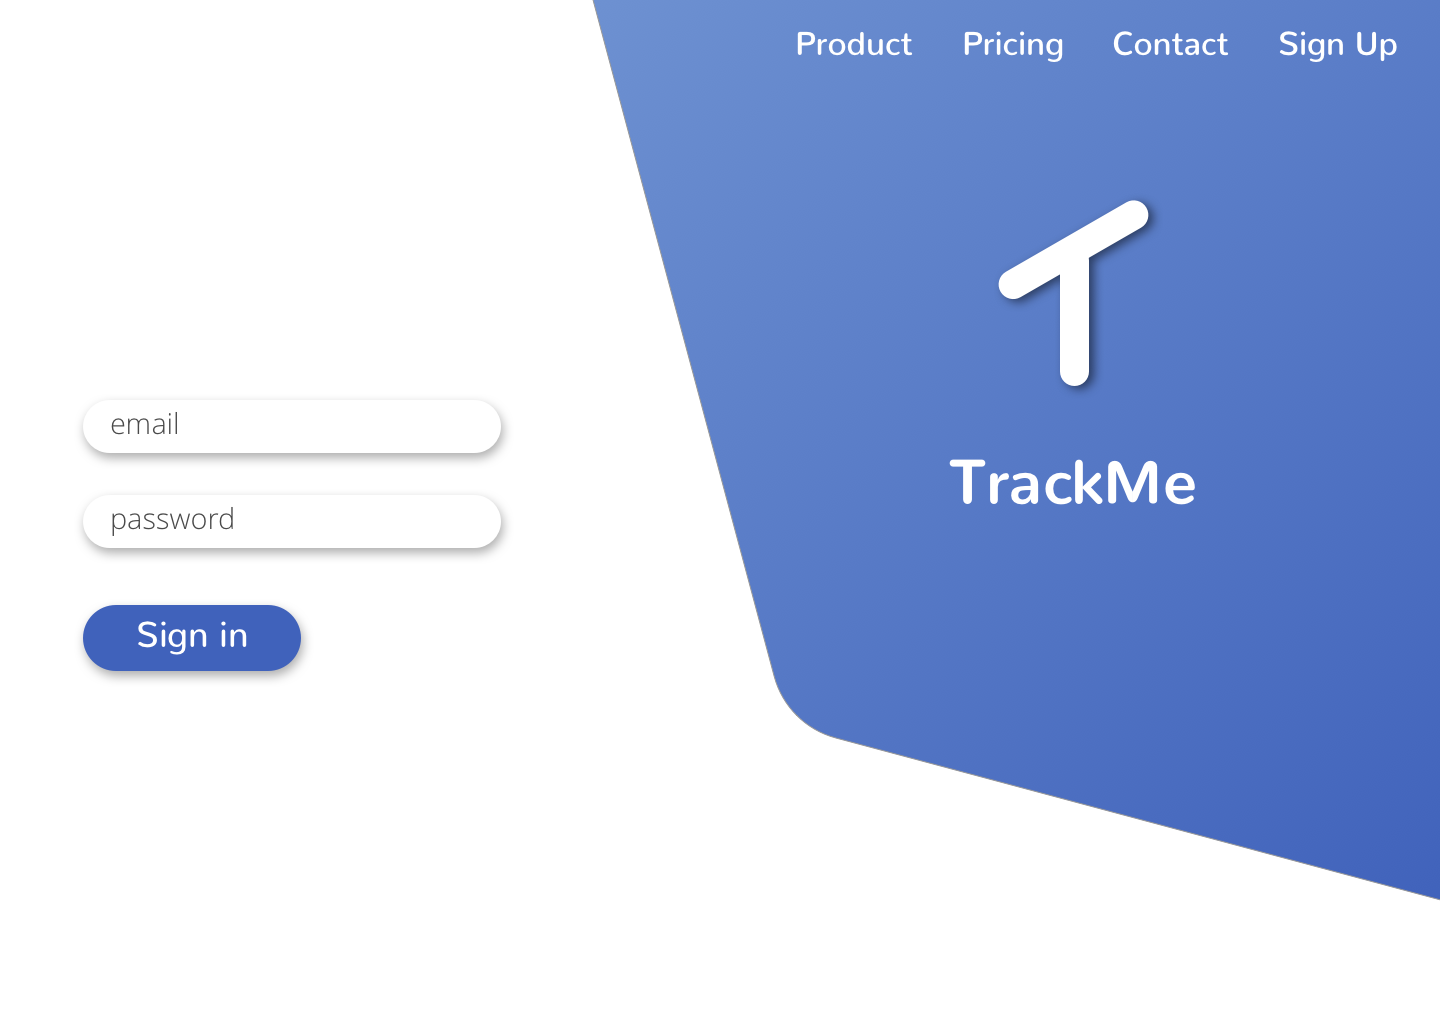
\includegraphics[scale=0.18]{./Pictures/Mockup/web/login.png}}
   
\end{figure}

\begin{figure}[H]

    \centering
    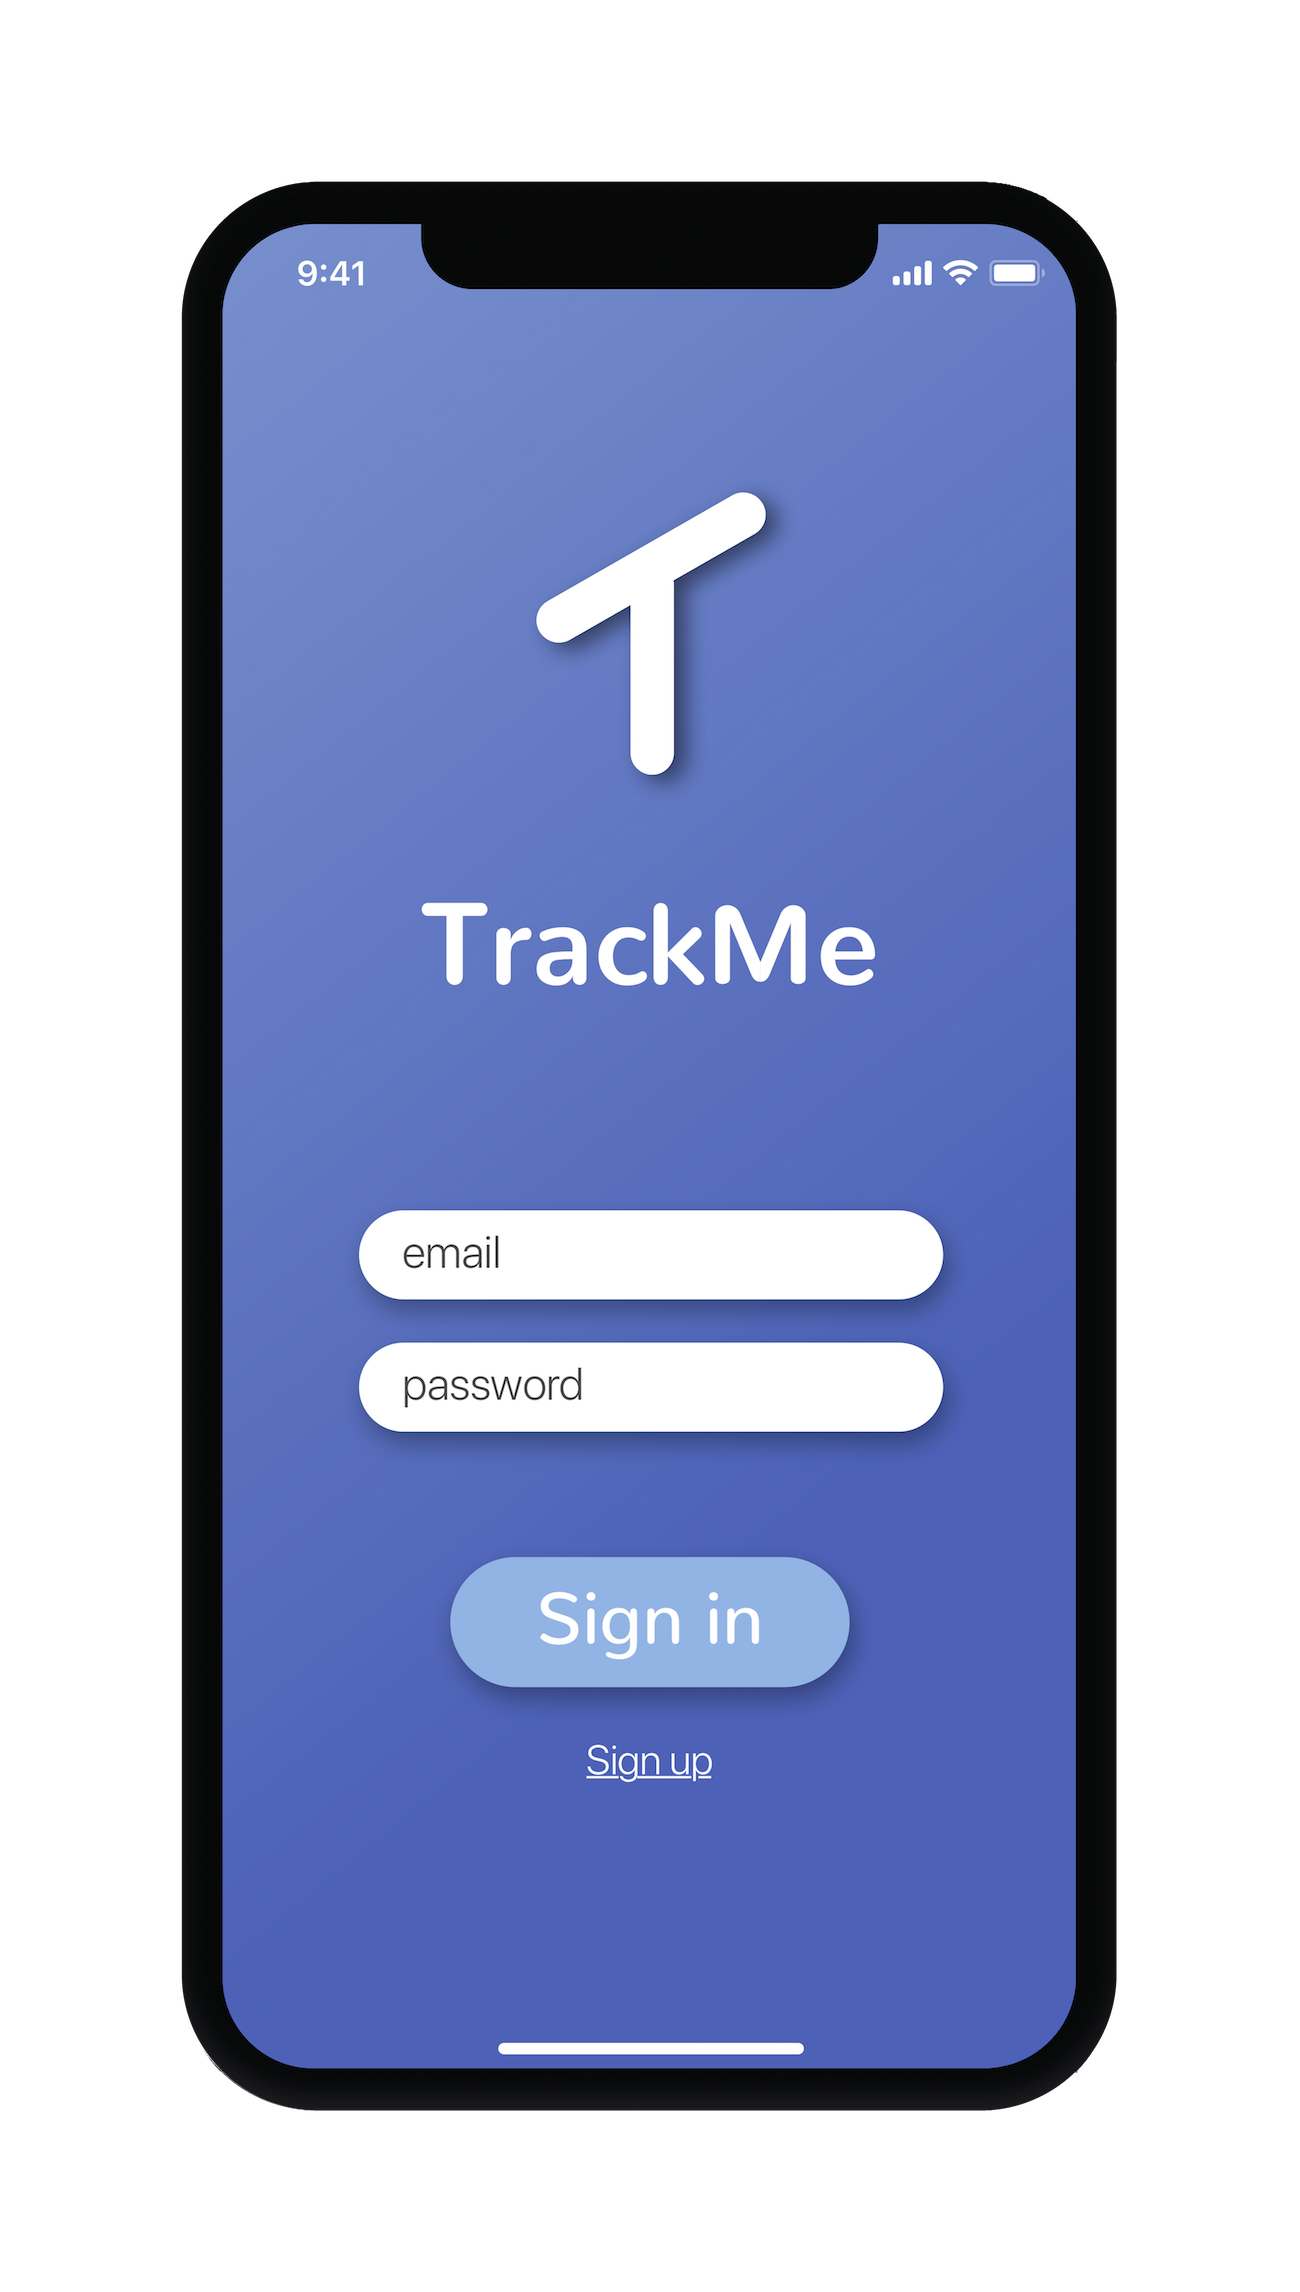
\includegraphics[width=0.30\textwidth]{./Pictures/Mockup/mobile/login.png}
    
\end{figure}

\section{UX Diagrams}
To explain how TrackMe users will interact with the system, UX diagrams of the Mobile application and the Web application are represented below.

\begin{figure}[H]

    \centering
    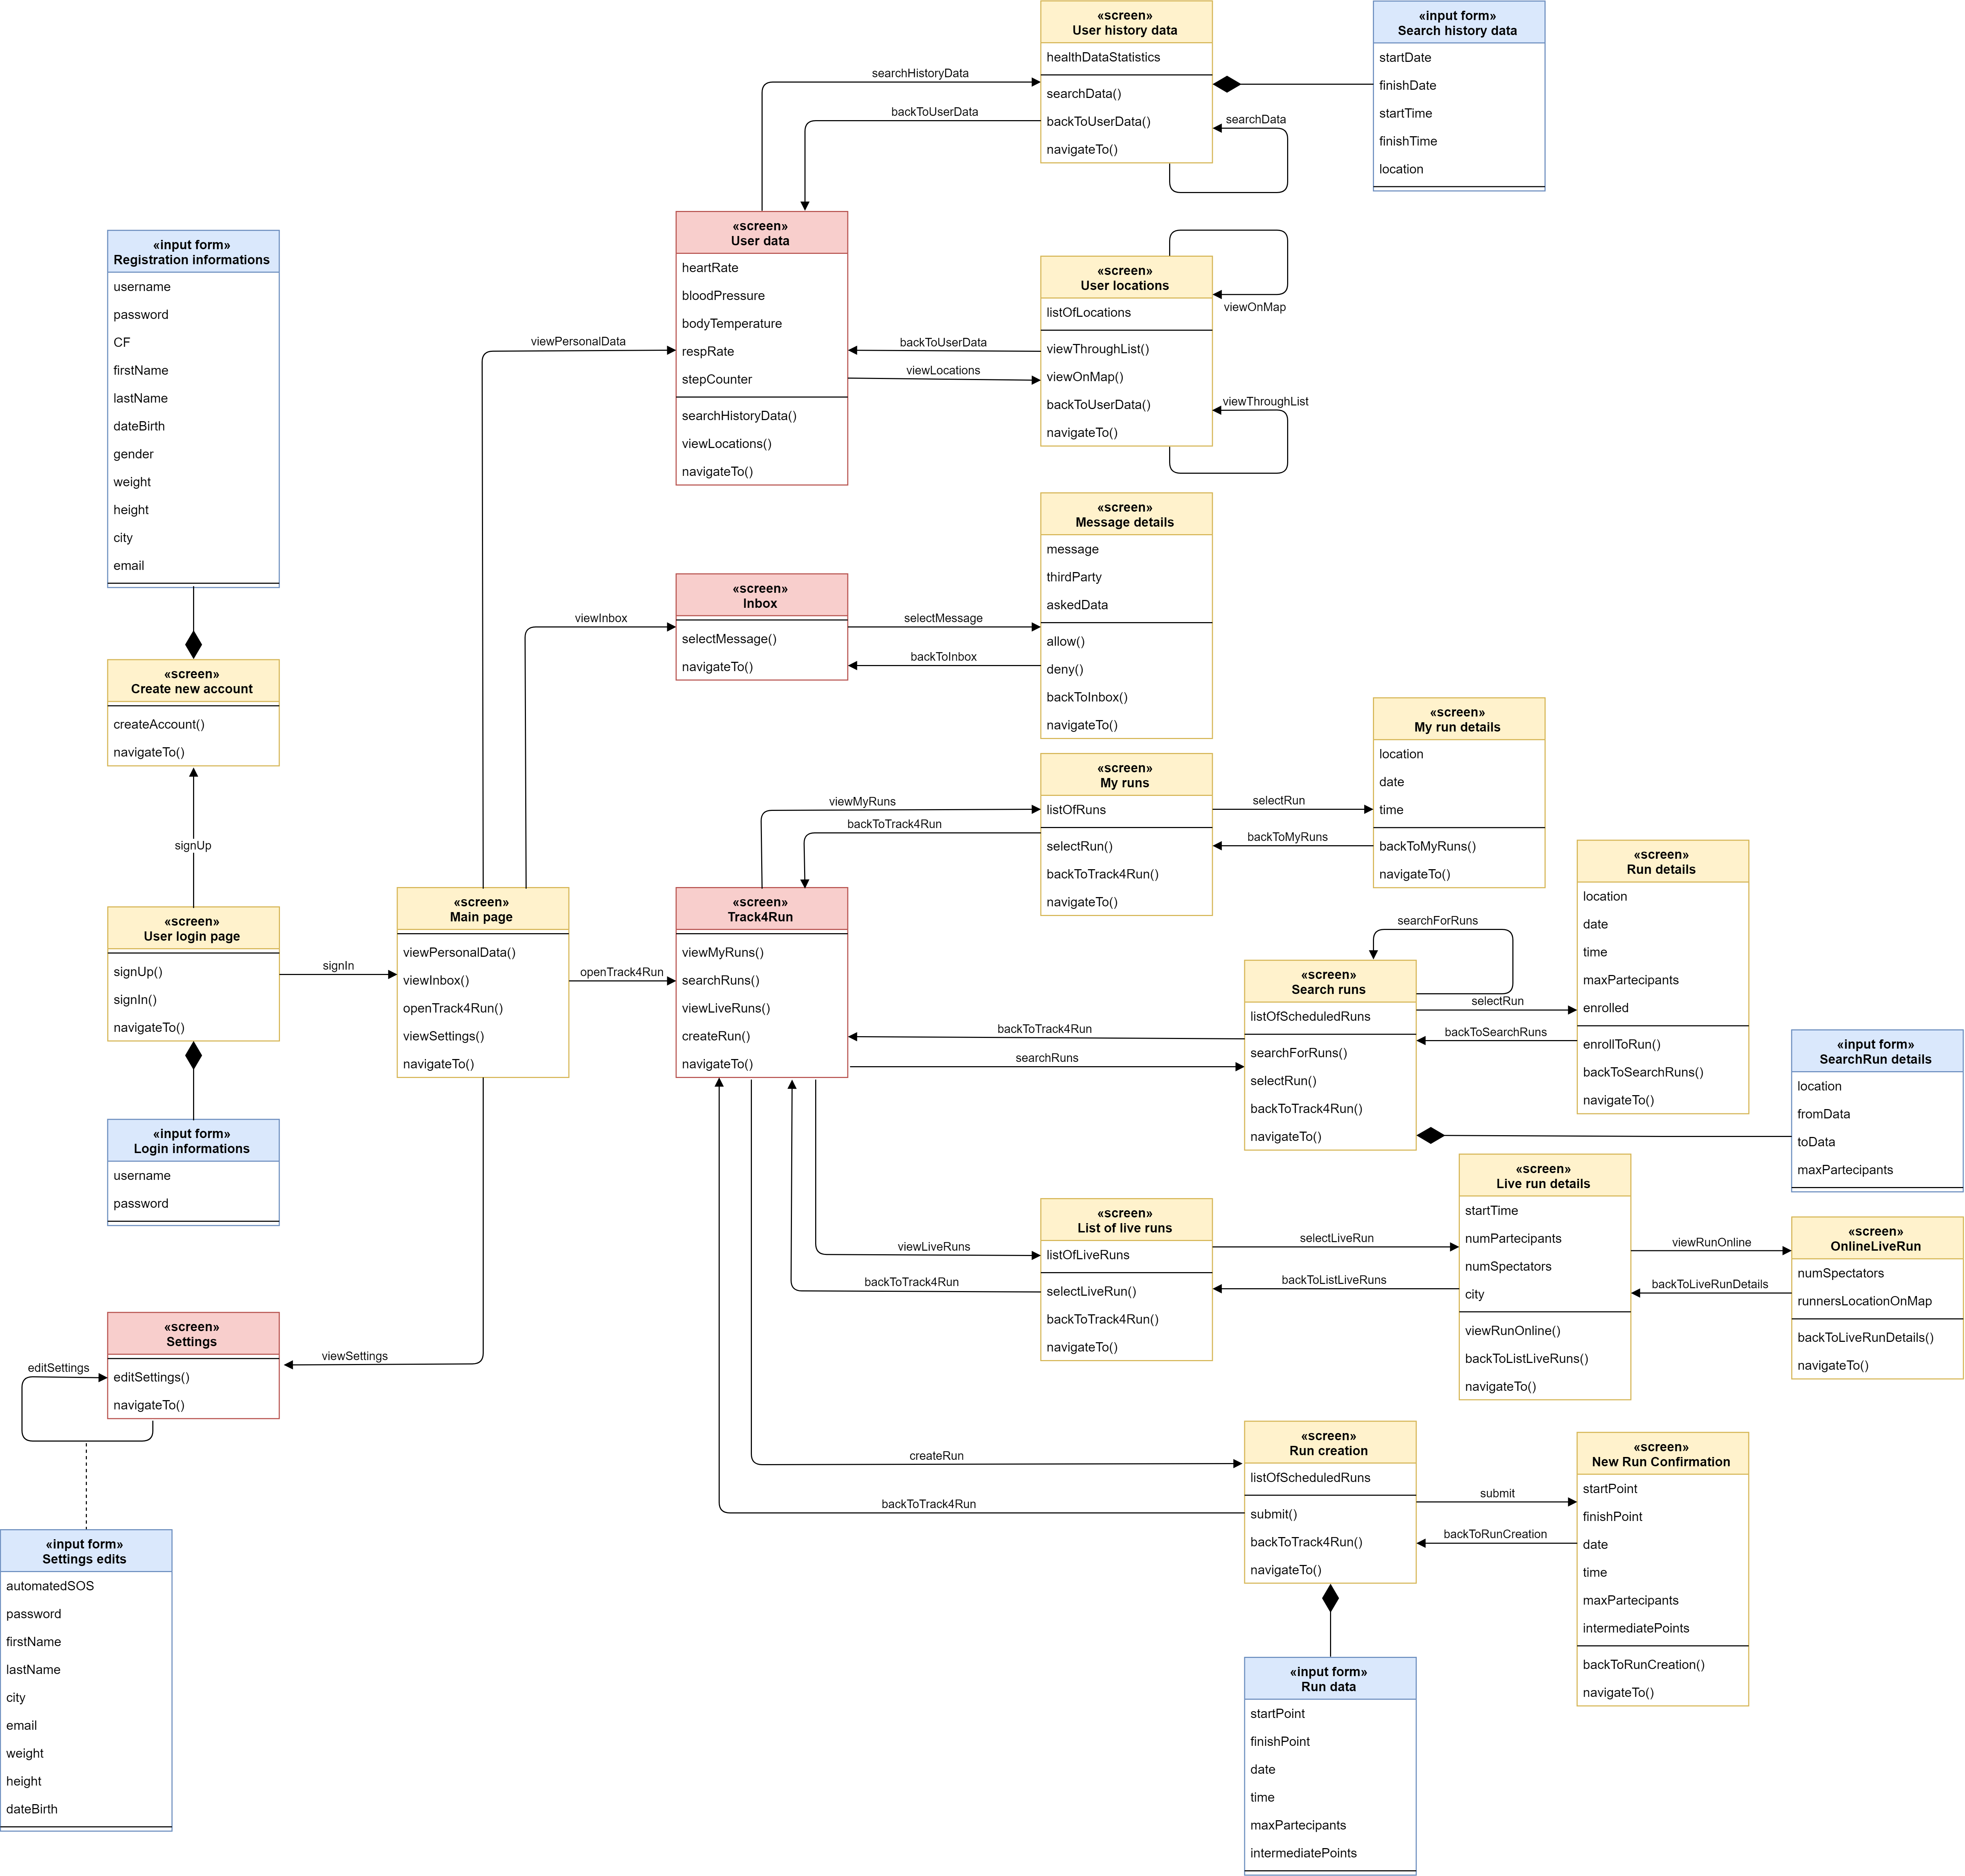
\includegraphics[width=1\textwidth]{./Pictures/UXMobile.png}
    \caption{UX diagram of the User Mobile application}
    
\end{figure}

\begin{figure}[H]

    \centering
    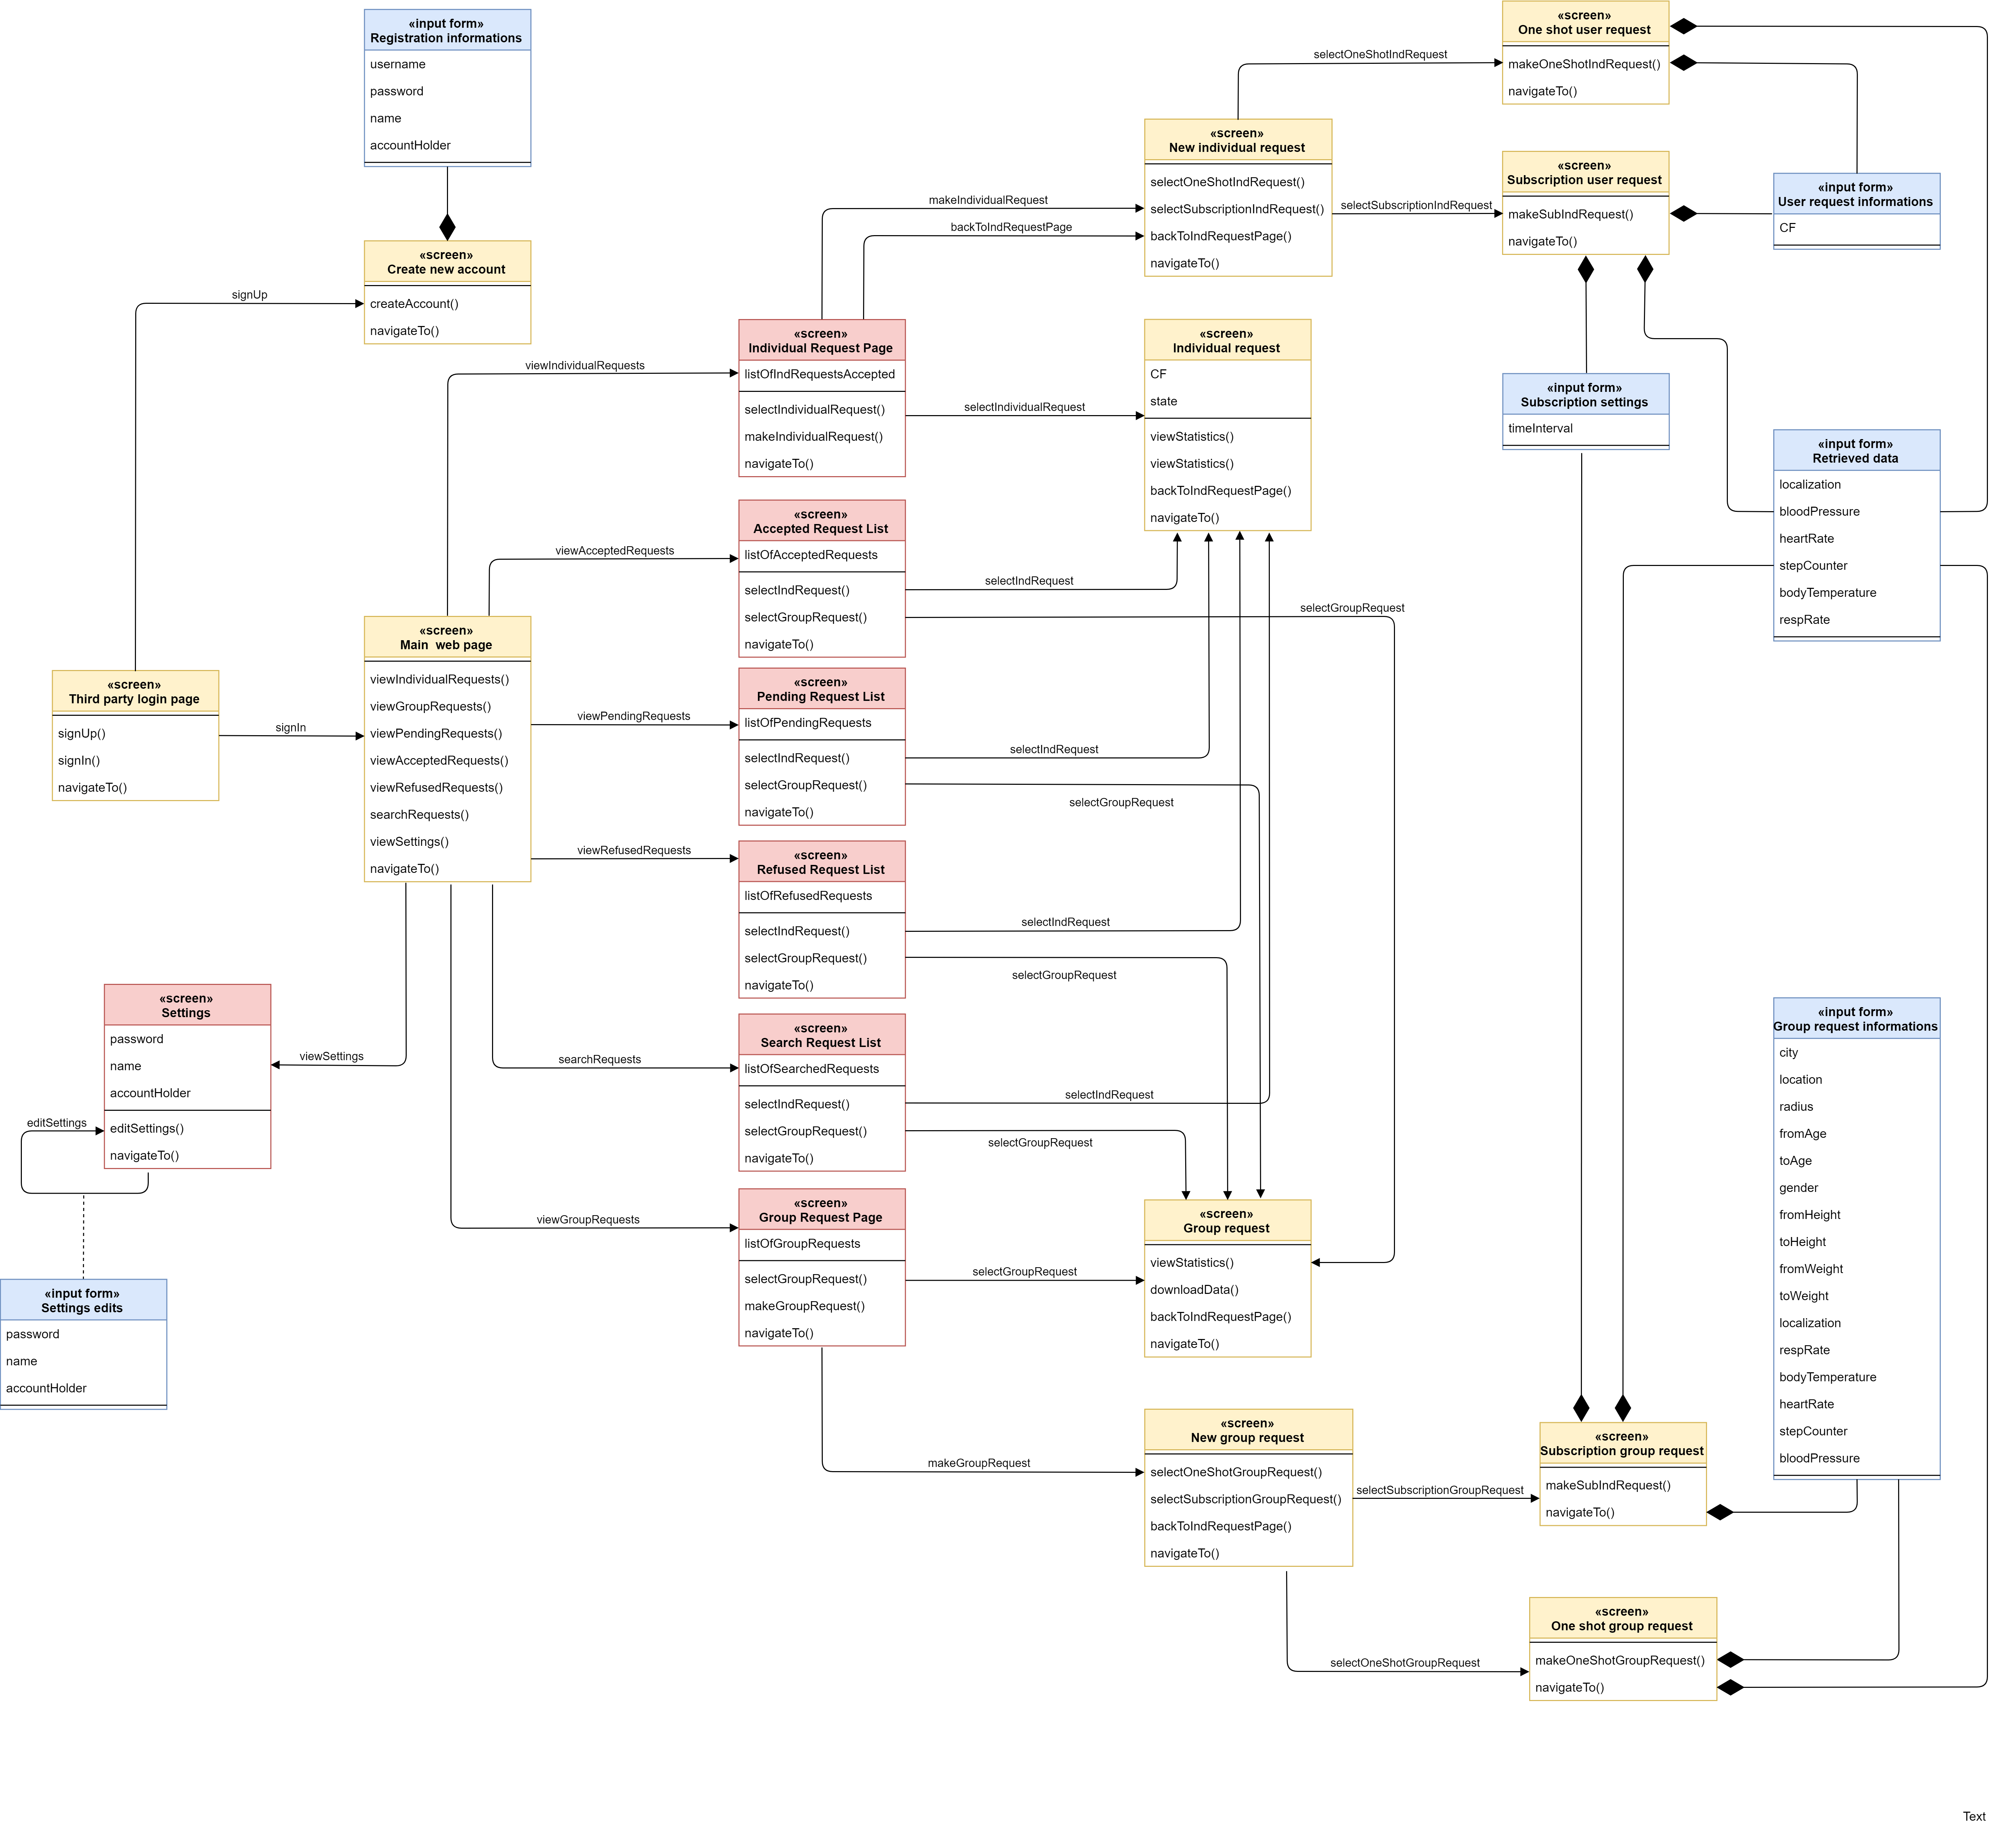
\includegraphics[width=1\textwidth]{./Pictures/UXWeb.png}
    \caption{UX diagram of the Third Party Web application}
    
\end{figure}

The screens in red of the UX diagrams are the parts of the application that are always reachable from the bottom menu in the Mobile application and from the leftmost menu in the Web application. These screens are reachable from every page of the Mobile and Web application, except from the \textit{User login page}, \textit{Third Party login page} and the \textit{Create new account} screens.

\begin{figure}[H]

    \centering
    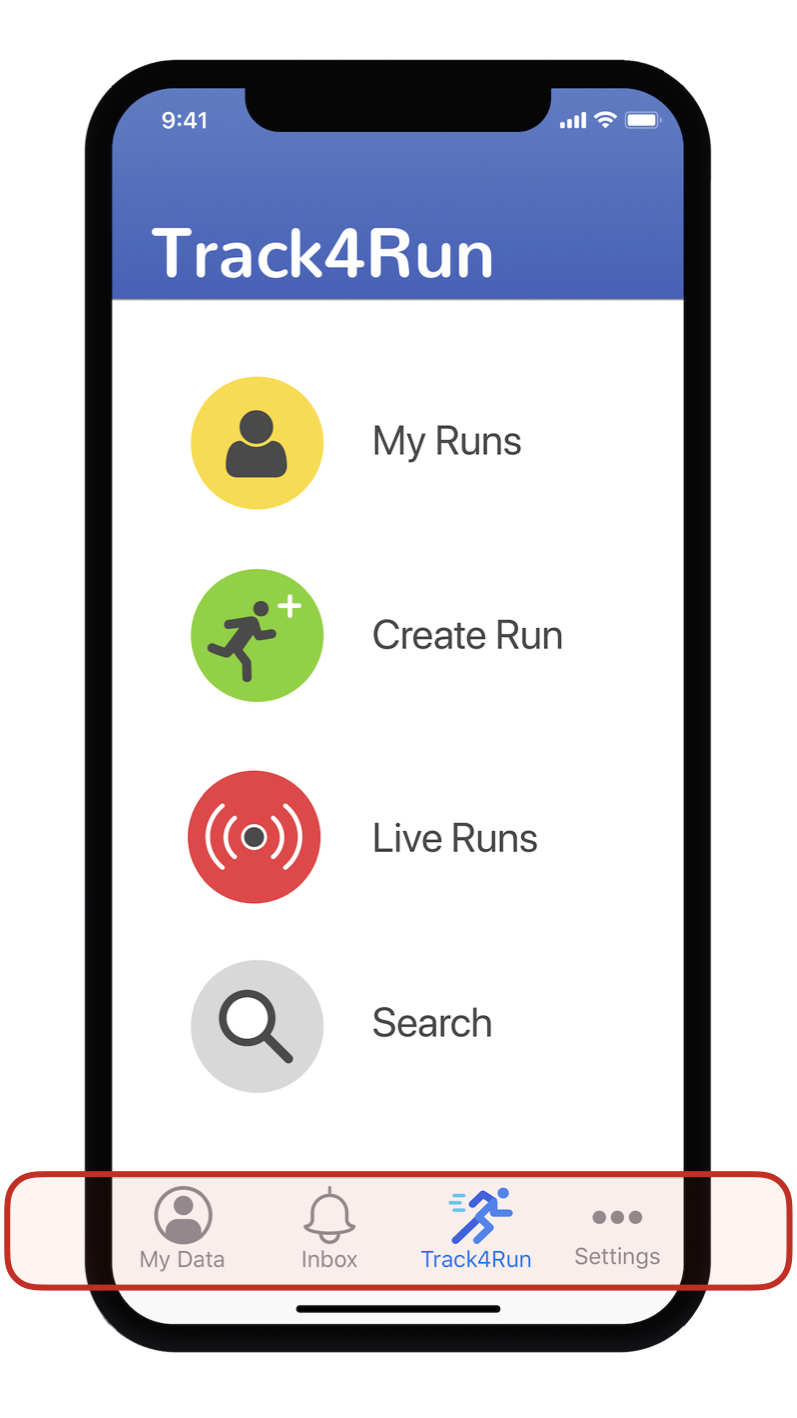
\includegraphics[width=0.3\textwidth]{./Pictures/ux-highlight-mobile.jpeg}
    \caption{Bottom menu from which it is possible to open My Data, Inbox, Track4Run and Settings in the Mobile application}
    
\end{figure}

\begin{figure}[H]

    \centering
    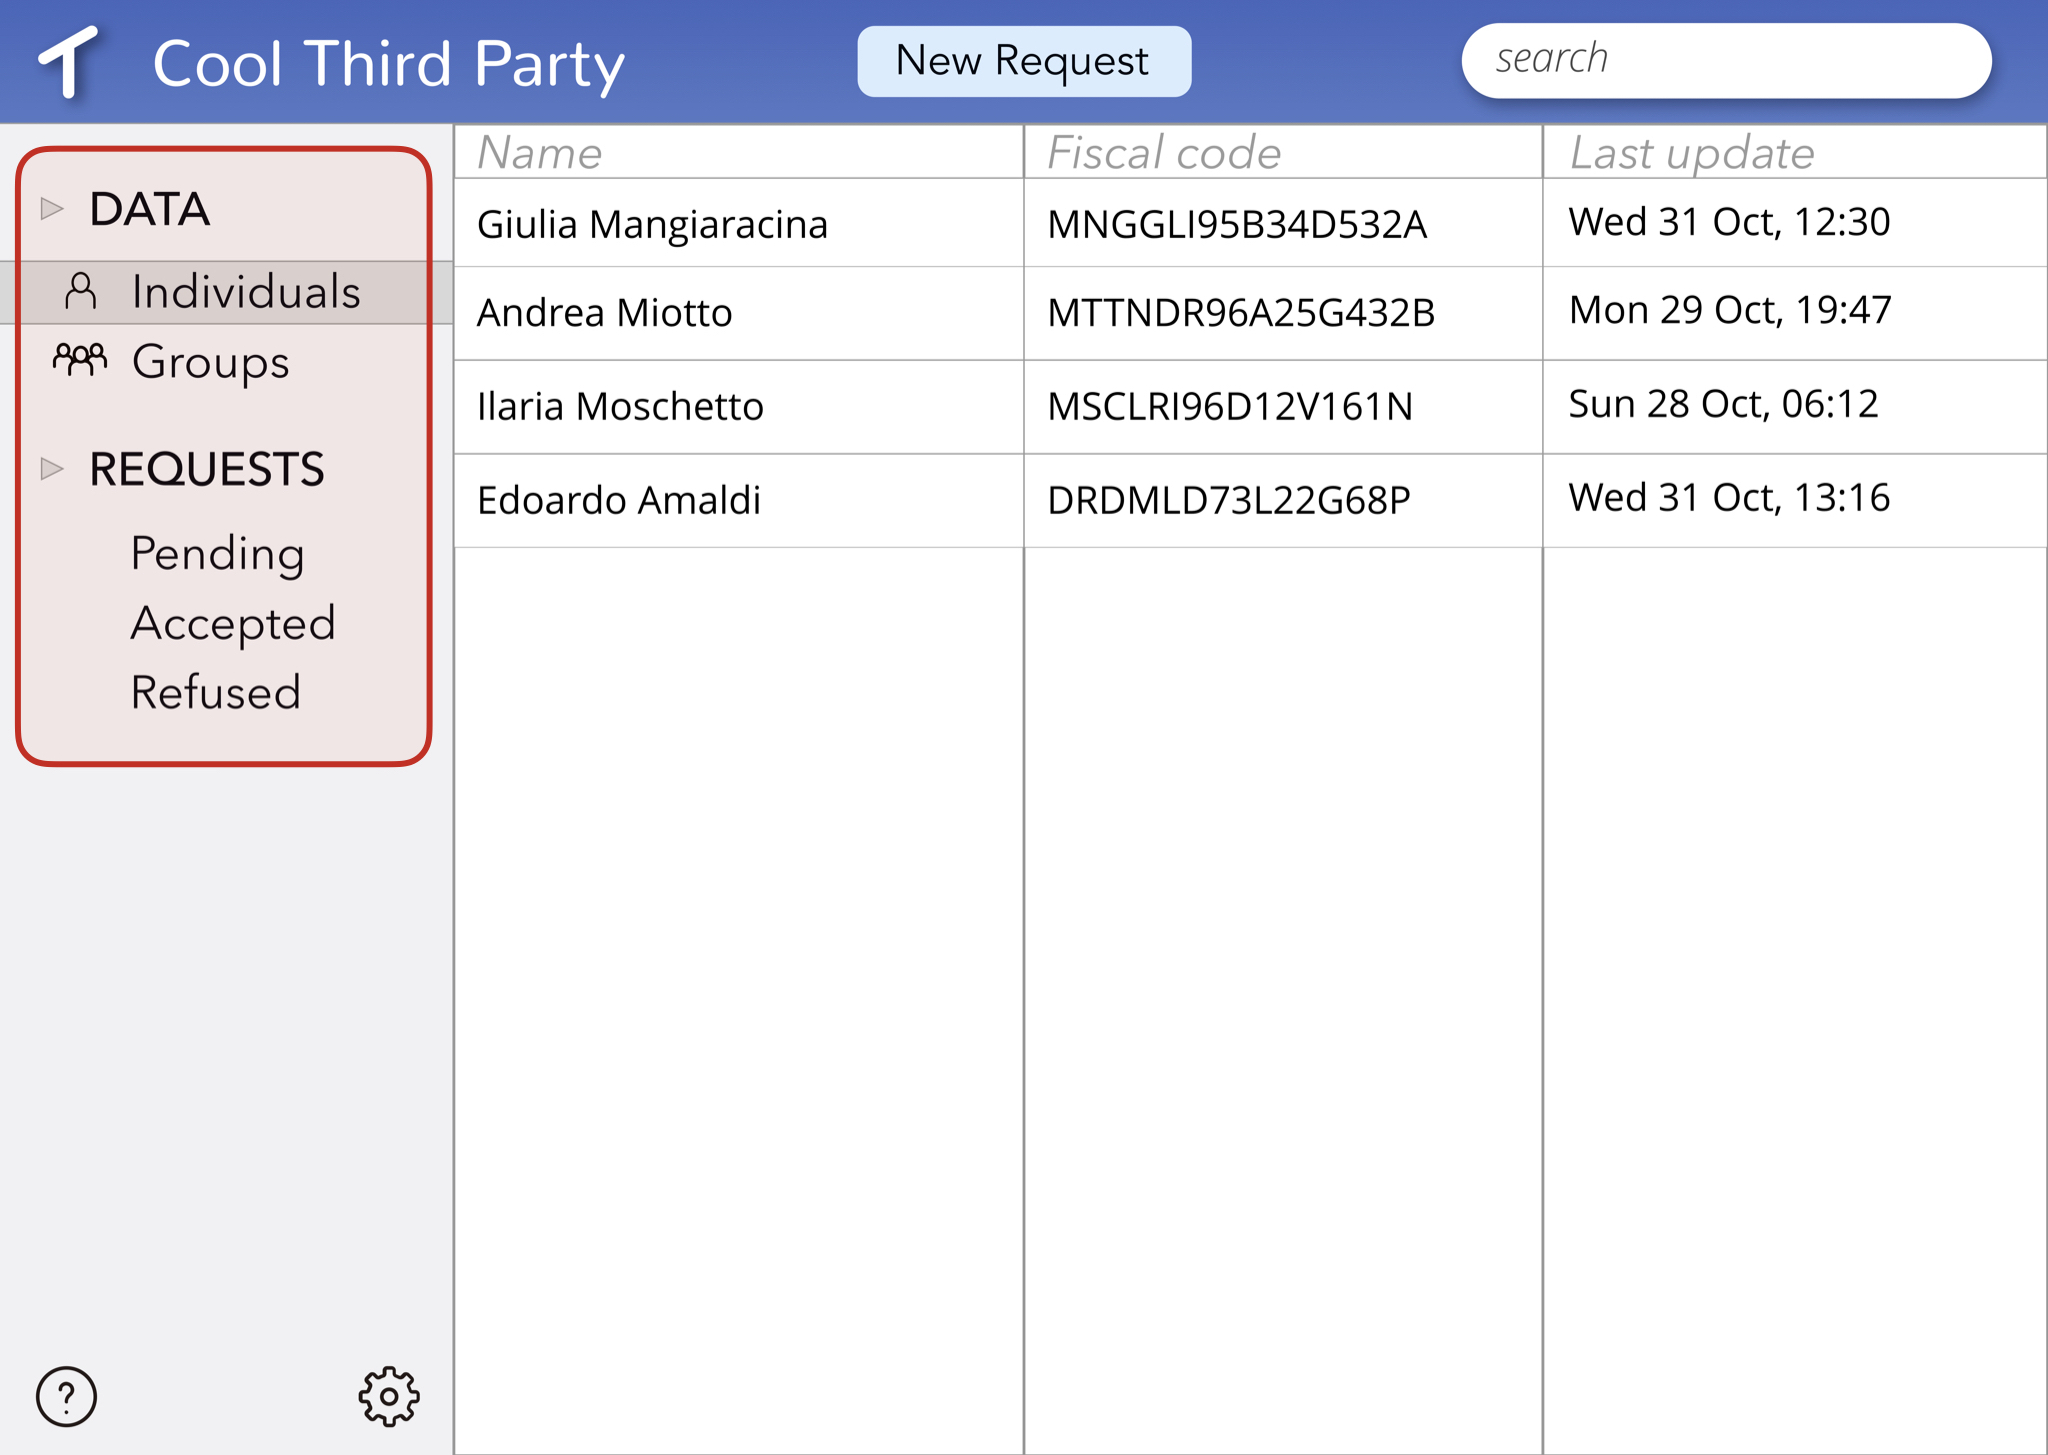
\includegraphics[width=0.7\textwidth]{./Pictures/ux-highlight-web.jpeg}
    \caption{Leftmost menu from which it is possible to open Individuals, Groups, Pending, Accepted and Refused requests views in the Web application}
    
\end{figure}